\section{Introduction}

%%%%% NEUTRINO PROPERTIES %%%%%

\begin{slide}[toc=Neutrino properties]{Basic properties of neutrinos}
  
  % elementary particles table
  \rput(0.8\slidewidth,0.0\slideheight){\scalebox{0.75}{% elementary particles table
\begin{pspicture}

  \psframe[linestyle = none, fillstyle = solid, fillcolor = pdcolor3](3,4)(3.8,4.8)\rput[c](3.4,4.4){\color{pdcolor2} $H$}

  \psframe[shadow = true, shadowsize = 0.05, shadowcolor = pdcolor3, linewidth = 0.01, linecolor = pdcolor1](0,3)(.8,3.8)\rput[c](0.4,3.4){\color{pdcolor1} $u$}
  \psframe[shadow = true, shadowsize = 0.05, shadowcolor = pdcolor3, linewidth = 0.01, linecolor = pdcolor1](1,3)(1.8,3.8)\rput[c](1.4,3.4){\color{pdcolor1} $c$}
  \psframe[shadow = true, shadowsize = 0.05, shadowcolor = pdcolor3, linewidth = 0.01, linecolor = pdcolor1](2,3)(2.8,3.8)\rput[c](2.4,3.4){\color{pdcolor1} $t$}
  \psframe[linestyle = none, fillstyle = solid, fillcolor = pdcolor1](3,3)(3.8,3.8)\rput[c](3.4,3.4){\color{pdcolor2} $\gamma$}
  
  \psframe[shadow = true, shadowsize = 0.05, shadowcolor = pdcolor3, linewidth = 0.01, linecolor = pdcolor1](0,2)(.8,2.8)\rput[c](0.4,2.4){\color{pdcolor1} $d$}
  \psframe[shadow = true, shadowsize = 0.05, shadowcolor = pdcolor3, linewidth = 0.01, linecolor = pdcolor1](1,2)(1.8,2.8)\rput[c](1.4,2.4){\color{pdcolor1} $s$}
  \psframe[shadow = true, shadowsize = 0.05, shadowcolor = pdcolor3, linewidth = 0.01, linecolor = pdcolor1](2,2)(2.8,2.8)\rput[c](2.4,2.4){\color{pdcolor1} $b$}
  \psframe[linestyle = none, fillstyle = solid, fillcolor = pdcolor1](3,2)(3.8,2.8)\rput[c](3.4,2.4){\color{pdcolor2} $g$}
  
  \psline[linewidth = 0.02, linestyle = dotted, linecolor = pdcolor1](0,1.875)(2.8,1.875)
  
  \psframe[shadow = true, shadowsize = 0.05, shadowcolor = pdcolor3, linewidth = 0.01, linecolor = pdcolor1](0,1)(.8,1.8)\rput[c](0.4,1.4){\color{pdcolor1} $\nu_e$}
  \psframe[shadow = true, shadowsize = 0.05, shadowcolor = pdcolor3, linewidth = 0.01, linecolor = pdcolor1](1,1)(1.8,1.8)\rput[c](1.4,1.4){\color{pdcolor1} $\nu_\mu$}
  \psframe[shadow = true, shadowsize = 0.05, shadowcolor = pdcolor3, linewidth = 0.01, linecolor = pdcolor1](2,1)(2.8,1.8)\rput[c](2.4,1.4){\color{pdcolor1} $\nu_\tau$}
  \psframe[linestyle = none, fillstyle = solid, fillcolor = pdcolor1](3,1)(3.8,1.8)\rput[c](3.4,1.4){\color{pdcolor2} $Z^0$}

  \psframe[shadow = true, shadowsize = 0.05, shadowcolor = pdcolor3, linewidth = 0.01, linecolor = pdcolor1](0,0)(.8,.8)\rput[c](0.4,0.4){\color{pdcolor1} $e$}
  \psframe[shadow = true, shadowsize = 0.05, shadowcolor = pdcolor3, linewidth = 0.01, linecolor = pdcolor1](1,0)(1.8,.8)\rput[c](1.4,0.4){\color{pdcolor1} $\mu$}
  \psframe[shadow = true, shadowsize = 0.05, shadowcolor = pdcolor3, linewidth = 0.01, linecolor = pdcolor1](2,0)(2.8,.8)\rput[c](2.4,0.4){\color{pdcolor1} $\tau$}
  \psframe[linestyle = none, fillstyle = solid, fillcolor = pdcolor1](3,0)(3.8,.8)\rput[c](3.4,0.4){\color{pdcolor2} $W^\pm$}
  
  \rput[c]{L}(-0.2,2.9){\footnotesize QUARKS}
  \rput[c]{L}(-0.2,0.9){\footnotesize LEPTONS}
  \rput[c]{R}(4, 1.9){\footnotesize BOSONS}
  \rput[c](1.4, 4.6){\scriptsize Three generations}
  \rput[c](1.4, 4.3){\scriptsize of fermions}
  \rput[c](0.4, 4){\footnotesize I}
  \rput[c](1.4, 4){\footnotesize II}
  \rput[c](2.4, 4){\footnotesize III}
  
\end{pspicture}
}}
  
  % neutrino oscillation
  \rput(0.15\slidewidth,-0.4\slideheight){\scalebox{0.5}{% neutrino oscillation
\begin{pspicture}
  
  \cnodeput[linestyle = none, fillstyle = solid, fillcolor = pdcolor1](0.5,0.57){nu1}{\Large\color{pdcolor2} $\nu_\alpha$}
    
  \psline[linewidth = 0.03, linecolor = pdcolor1](1.2, 0.57)(3.25, 0.57)
    
  \pscircle[linewidth = 0.03, linecolor = pdcolor1, linestyle = dotted](5, 0.57){1.75}
  \cnodeput[linestyle = none, fillstyle = solid, fillcolor = pdcolor7](5,1.7){nue}{\Large\color{pdcolor2} $\nu_e$}
  \cnodeput[linestyle = none, fillstyle = solid, fillcolor = pdcolor4](4,0){num}{\Large\color{pdcolor2} $\nu_\mu$}
  \cnodeput[linestyle = none, fillstyle = solid, fillcolor = pdcolor6](6,0){nut}{\Large\color{pdcolor2} $\nu_\tau$}

  \psline[linewidth = 0.03, linecolor = pdcolor1]{->}(6.75, 0.57)(8.8, 0.57)

  \cnodeput[linestyle = none, fillstyle = solid, fillcolor = pdcolor1](9.5,0.57){nu1}{\Large\color{pdcolor2} $\nu_\beta$}

  \psset{nodesep = 3pt}
  \ncarc[linecolor = pdcolor4]{->}{nue}{num}
  \ncarc[linecolor = pdcolor7]{->}{num}{nue}
  \ncarc[linecolor = pdcolor6]{->}{num}{nut}
  \ncarc[linecolor = pdcolor4]{->}{nut}{num}
  \ncarc[linecolor = pdcolor7]{->}{nut}{nue}
  \ncarc[linecolor = pdcolor6]{->}{nue}{nut}

\end{pspicture}
}}
  
  \vspace{-20pt}  
  \begin{itemize}

    \item $\frac{1}{2}$-spin, no electric charge, small mass \\ (extremely hard to detect)
    
    \item Interactions with elementary particles \\ $\rightarrow$ electroweak theory (Standard Model)
    
    \item Interactions with nucleons \\ $\rightarrow$ form factors \\ $\rightarrow$ parton distribution functions
    
    \item Interactions with nuclei $\rightarrow$ nuclear effects
        
    \item The neutrino flavor state is a superposition of the mass states: \\ \vspace{10pt}
    \hspace{160pt}$\left|\nu_\alpha\right> = \sum_i U_{\alpha i} \left|\nu_i\right>$
    \vspace{10pt}
    
    \hspace{125pt}The neutrino produced in $\alpha$ state \\ \hspace{125pt}can be measured in $\beta$ state.\\ \hspace{125pt}The phenomenon is called \\ \hspace{125pt}neutrino oscillation.
    
  \end{itemize}
    
\end{slide}

%%%%% PMNS MATRIX %%%%%

\begin{wideslide}[toc=PMNS matrix]{Pontecorvo-Maki-Nakagawa-Sakata matrix}
  
  The PMNS matrix defines the mass mixing in the lepton sector:
  
  $$U =    
    \left[\begin{array}{ccc}
      1 & 0 & 0 \\ 
      0 & \grey{c_{23}} & \grey{s_{23}} \\ 
      0 & -\grey{s_{23}} & \grey{c_{23}}
    \end{array}\right]
    \left[\begin{array}{ccc}
      \grey{c_{13}} & 0 & \grey{s_{13}}\red{e^{-i\delta}} \\
      0 & 1 & 0 \\
      -\grey{s_{13}}\red{e^{i\delta}} & 0 & \grey{c_{13}}
    \end{array}\right]  
    \left[\begin{array}{ccc}
      \grey{c_{12}} & \grey{s_{12}} & 0 \\
      -\grey{s_{12}} & \grey{c_{12}} & 0 \\
      0 & 0 & 1
    \end{array}\right]
  $$
  
  \mbox{}\vspace{5pt}
  
  \makebox[\textwidth]{\grey{$c_{ij} = \cos\theta_{ij}$ \hspace{10pt} $s_{ij} = \sin\theta_{ij}$ \hspace{10pt} $\theta_{ij}$ - mixing angels} \hspace{10pt} \red{$\delta$ - CP phase factor}}

  \psline[linewidth = 0.01, linecolor = pdcolor1](-5,0.225)(15,0.225)
  \psline[linewidth = 0.01, linecolor = pdcolor1](-5,0.825)(15,0.825)
 
  \begin{center}
    Measurements:
  \end{center}
 
  \mbox{}%\vspace{10pt}
   
  \begin{minipage}{0.5\columnwidth}
    \begin{itemize}
      \item Solar, reactor and accelerator:
      \item Atmospheric:
      \item Reactor:
    \end{itemize}
  \end{minipage}
  \begin{minipage}{0.4\columnwidth}
    \begin{itemize}
      \item[] $\grey{\sin^2(2\theta_{12}) = 0.846 \pm 0.021}$
      \item[] $\grey{\sin^2(2\theta_{23}) > 0.92}$
      \item[] $\grey{\sin^2(2\theta_{13}) = 0.093 \pm 0.008}$
    \end{itemize} 
  \end{minipage}
  \mbox{}\vspace{15pt}
  \makebox[\textwidth]{$\red{\delta}$ can be measured if and only if all mixing angles are nonzero. If $\red{\delta \neq 0}$ CP is violated.}
  
  \psline[linewidth = 0.01, linecolor = pdcolor1](-5,0.25)(15,0.25)
  \psline[linewidth = 0.01, linecolor = pdcolor1](-5,0.85)(15,0.85)
  
\end{wideslide}

%%%%% PROBABILITY OF OSCILLATION %%%%%

\begin{slide}{Probability of oscillation}
    
  \begin{eqnarray*}
    P(\nu_\alpha \rightarrow \nu_\beta)
      & = & \left|\left<\nu_\beta(x)|\nu_\alpha(y)\right>\right|^2 = \delta_{\alpha\beta} \\
      & - & 4 \sum_{i>j}\Re\left[U^*_{\alpha i}U_{i\beta}U_{\alpha_j}U^*_{j\beta}\right]\sin^2\left(\frac{{\blue{\Delta m_{ij}}^2} \grey{L}}{4\red{E}}\right) \\ 
      & + & 2\sum_{i>j}\Im\left[U^*_{\alpha i}U_{i\beta}U_{\alpha_j}U^*_{j\beta}\right]\sin^2\left(\frac{{\blue{\Delta m_{ij}}^2} \grey{L}}{2\red{E}}\right)
  \end{eqnarray*}
  
  \psframe[linewidth = 0.01, linecolor = pdcolor1](-0.7,1.8)(2.7,1.2)
  \rput[c](1,1.5){\blue{$\Delta m_{ij}^2 \equiv m_i^2 - m_j^2$}}

  \mbox{} \vspace{5pt}
  
  \grey{$L$} - traveled distance (fixed), \red{$E$} - neutrino energy (will be discussed)
  
  \psline[linewidth = 0.01, linecolor = pdcolor1](-0.8,0)(10.7,0)
  \psline[linewidth = 0.01, linecolor = pdcolor1](-0.8,1)(10.7,1)
      
  \begin{center}
    Measurements:
  \end{center}
 
  \mbox{}%\vspace{10pt}
   
  \begin{minipage}{0.4\columnwidth}
    \begin{itemize}
      \item Solar neutrinos:
      \item Atmospheric neutrinos:
    \end{itemize}
  \end{minipage}
  \begin{minipage}{0.575\columnwidth}
    \begin{itemize}
      \item[] \blue{$\Delta m^2_{21} = (7.53 \pm 0.18) \cdot 10^{-5} eV^2$}
      \item[] \blue{$|\Delta m^2_{32}| = (2.44 \pm 0.06) \cdot 10^{-3} eV^2$}
    \end{itemize} 
  \end{minipage}

  
\end{slide}

%%%%% MASS HIERARCHY AND CPT %%%%%

\begin{wideslide}{Neutrino oscillation}
   
  % mass hierarchy 
  \rput(0.95\slidewidth, 0.05\slideheight){\scalebox{0.75}{% mass hierarchy
\begin{pspicture}
  
  \rput[c](0.8,3.7){\color{pdcolor1}\small\it Normal hierarchy}
  \psframe[linestyle = none, fillstyle = solid, fillcolor = pdcolor6](0,3)(2,3.2)\rput[r](-0.1,3.1){\color{pdcolor6} $m_3^2$}
  \psline[linewidth = 0.05, linecolor = pdcolor1, arrowinset = 0.1]{<->}(1, 1.2)(1, 3)\rput[l](1.1, 2.1){\color{pdcolor1} $\Delta m_{32}^2$}
  \psframe[linestyle = none, fillstyle = solid, fillcolor = pdcolor7](0,1)(2,1.2)\rput[r](-0.1,1.1){\color{pdcolor7} $m_2^2$}
  \psline[linewidth = 0.05, linecolor = pdcolor1, arrowinset = 0.1]{<->}(1, 0.2)(1, 1)\rput[l](1.1, 0.6){\color{pdcolor1} $\Delta m_{21}^2$}
  \psframe[linestyle = none, fillstyle = solid, fillcolor = pdcolor4](0,0)(2,0.2)\rput[r](-0.1,0.1){\color{pdcolor4} $m_1^2$}
  \psline[linewidth = 0.05, linecolor = pdcolor1, arrowinset = 0.1]{<->}(1, -0.8)(1, 0)\rput[l](1.1, -0.4){\color{pdcolor1} ?}
  \psframe[linestyle = none, fillstyle = solid, fillcolor = pdcolor1](0,-1)(2,-0.8)\rput[r](-0.1,-0.9){\color{pdcolor1} $0$}

  \rput[c](3.8,3.7){\color{pdcolor1}\small\it Inverted hierarchy}
  \psframe[linestyle = none, fillstyle = solid, fillcolor = pdcolor7](3,3)(5,3.2)\rput[r](2.9,3.1){\color{pdcolor7} $m_2^2$}
  \psline[linewidth = 0.05, linecolor = pdcolor1, arrowinset = 0.1]{<->}(4, 2.2)(4, 3)\rput[l](4.1, 2.6){\color{pdcolor1} $\Delta m_{21}^2$}
  \psframe[linestyle = none, fillstyle = solid, fillcolor = pdcolor4](3,2)(5,2.2)\rput[r](2.9,2.1){\color{pdcolor4} $m_1^2$}
  \psline[linewidth = 0.05, linecolor = pdcolor1, arrowinset = 0.1]{<->}(4, 0.2)(4, 2)\rput[l](4.1, 1.1){\color{pdcolor1} $\Delta m_{31}^2$}
  \psframe[linestyle = none, fillstyle = solid, fillcolor = pdcolor6](3,0)(5,0.2)\rput[r](2.9,0.1){\color{pdcolor6} $m_3^2$}
  \psline[linewidth = 0.05, linecolor = pdcolor1, arrowinset = 0.1]{<->}(4, -0.8)(4, 0)\rput[l](4.1, -0.4){\color{pdcolor1} ?}
  \psframe[linestyle = none, fillstyle = solid, fillcolor = pdcolor1](3,-1)(5,-0.8)\rput[r](2.9,-0.9){\color{pdcolor1} $0$}

\end{pspicture}
}}
  
  % CPT
  \rput(0.35\slidewidth, -0.4\slideheight){\scalebox{0.75}{% CPT figure
\begin{pspicture}

  \psset{nodesep = 3pt}

  \cnode[linestyle = none, fillstyle = solid, fillcolor = pdcolor1](0,3.5){0.35}{c1}
  \rput[c](0,3.5){\color{pdcolor2} $+$}
  \psarc[linecolor = pdcolor2, fillstyle = none, arrowinset = 0]{->}(0,3.5){.25}{135}{405}
  \psline[linecolor = pdcolor1, linewidth = 0.05, arrowinset = 0.1]{->}(0,3.85)(0, 4.2)

  \cnode[linestyle = none, fillstyle = solid, fillcolor = pdcolor1](2,3.5){0.35}{c2}
  \rput[c](2,3.5){\color{pdcolor2} $-$}
  \psarc[linecolor = pdcolor2, fillstyle = none, arrowinset = 0]{->}(2,3.5){.25}{135}{405}
  \psline[linecolor = pdcolor1, linewidth = 0.05, arrowinset = 0.1]{->}(2,3.85)(2, 4.2)

  \ncarc[linecolor = pdcolor1]{<->}{c1}{c2}
  \naput{C}
  
  \rput[c](1, 2.9){\color{pdcolor1}\small charge conjugation}

  \cnode[linestyle = none, fillstyle = solid, fillcolor = pdcolor1](0,2){0.35}{p1}
  \rput[c](0,2){\color{pdcolor2} $+$}
  \psarc[linecolor = pdcolor2, fillstyle = none, arrowinset = 0]{->}(0,2){.25}{135}{405}
  \psline[linecolor = pdcolor1, linewidth = 0.05, arrowinset = 0.1]{->}(0,2.35)(0, 2.7)

  \cnode[linestyle = none, fillstyle = solid, fillcolor = pdcolor1](2,2){0.35}{p2}
  \rput[c](2,2){\color{pdcolor2} $+$}
  \psarc[linecolor = pdcolor2, fillstyle = none, arrowinset = 0]{<-}(2,2){.25}{135}{405}
  \psline[linecolor = pdcolor1, linewidth = 0.05, arrowinset = 0.1]{->}(2,2.35)(2, 2.7)

  \ncarc[linecolor = pdcolor1]{<->}{p1}{p2}
  \naput{P}  

  \rput[c](1, 1.4){\color{pdcolor1}\small parity transformation}
  
  \cnode[linestyle = none, fillstyle = solid, fillcolor = pdcolor1](0,0.5){0.35}{t1}
  \rput[c](0,0.5){\color{pdcolor2} $+$}
  \psarc[linecolor = pdcolor2, fillstyle = none, arrowinset = 0]{->}(0,0.5){.25}{135}{405}
  \psline[linecolor = pdcolor1, linewidth = 0.05, arrowinset = 0.1]{->}(0,0.85)(0, 1.2)

  \cnode[linestyle = none, fillstyle = solid, fillcolor = pdcolor1](2,0.5){0.35}{t2}
  \rput[c](2,0.5){\color{pdcolor2} $+$}
  \psarc[linecolor = pdcolor2, fillstyle = none, arrowinset = 0]{<-}(2,0.5){.25}{135}{405}
  \psline[linecolor = pdcolor1, linewidth = 0.05, arrowinset = 0.1]{->}(2,0.15)(2, -0.2)

  \ncarc[linecolor = pdcolor1]{<->}{t1}{t2}
  \naput{T}  
  
  \rput[c](1, -0.1){\color{pdcolor1}\small time reversal}

\end{pspicture}
}}

  \vspace{-15pt}
  \underline{The probability of neutrino oscillation depends on:}\\ \vspace{5pt}

  \begin{itemize}    
    \item What we want to measure:
    \begin{itemize}
      \item three mixing angles - already measured
      \item the difference between squared mass of the mass \\ states - the sign of $\Delta m_{32}^2$ is still unknown, \\what is the mass hierarchy?
      \item the CP phase factor - is the CP symmetry broken? \\ \vspace{5pt}\hspace{15pt}
      {\small$P(\bar\nu_\alpha \rightarrow \bar\nu_\beta) = P(\nu_\beta \rightarrow \nu_\alpha) \stackrel{?}{=} P(\nu_\alpha \rightarrow \nu_\beta)$}
    \end{itemize}

    \addtolength{\itemindent}{120pt}
    \vspace{10pt}

    \item What we need to know:
    
    \begin{itemize}
      \addtolength{\itemindent}{120pt}
      \item the distance traveled by a neutrino
      \item {\bf neutrino energy} - this is a problem      
    \end{itemize}
  
  \end{itemize}

\end{wideslide}

%%%%% MEASUREMENT IDEA %%%%%

\begin{slide}[toc=Measurement idea]{How to measure neutrino oscillation?}
 
 \rput(0.43\slidewidth, 0.33\slideheight){% oscillation measurement idea
\begin{pspicture}
  
  \rput[c](0,1.2){\color{pdcolor1} Neutrino source}
  \pscircle[linewidth = 0.05, linecolor = pdcolor1](0,0){0.9}
  \pscircle[linewidth = 0.05, linecolor = pdcolor1](0,0){0.65}
  {
  \psset{arrows = ->, arrowinset = 0}
  \psarc[linewidth = 0.03, linecolor = pdcolor1](0,0){0.75}{0}{60}
  \psarc[linewidth = 0.03, linecolor = pdcolor1](0,0){0.75}{60}{120}
  \psarc[linewidth = 0.03, linecolor = pdcolor1](0,0){0.75}{120}{180}
  \psarc[linewidth = 0.03, linecolor = pdcolor1](0,0){0.75}{180}{240}
  \psarc[linewidth = 0.03, linecolor = pdcolor1](0,0){0.75}{240}{300}
  \psarc[linewidth = 0.03, linecolor = pdcolor1](0,0){0.75}{300}{360}
  }
  \rput[c](0,0){\Large\color{pdcolor1} $\nu_\alpha$}
	
  \psline[linewidth = 0.03, linecolor = pdcolor1](1.2, 0)(2.25, 0)
    
  \pscircle[linewidth = 0.03, linecolor = pdcolor1, linestyle = dotted](4, 0){1.75}
  \cnodeput[linestyle = none, fillstyle = solid, fillcolor = pdcolor7](4,1.13){nue}{\Large\color{pdcolor2} $\nu_e$}
  \cnodeput[linestyle = none, fillstyle = solid, fillcolor = pdcolor4](3,-0.57){num}{\Large\color{pdcolor2} $\nu_\mu$}
  \cnodeput[linestyle = none, fillstyle = solid, fillcolor = pdcolor6](5,-0.57){nut}{\Large\color{pdcolor2} $\nu_\tau$}

  \psline[linewidth = 0.03, linecolor = pdcolor1]{->}(5.75, 0)(6.8, 0)
  
  \rput[c](7.9,1.2){\color{pdcolor1} Detector}
  \psframe[linewidth = 0.05, linecolor = pdcolor1](7,-0.9)(8.8,0.9)

  \psset{arrows = ->, arrowinset = 0.2}
  \psline[linewidth = 0.03, linecolor = pdcolor5]{->}(7.5, 0)(8.3, 0.5)
  \rput[c]{45}(7.75,0.45){\color{pdcolor5}$\alpha / \alpha'$}
  \psline[linewidth = 0.03, linecolor = pdcolor3]{->}(7.5, 0)(8.3, -0.1)
  \psline[linewidth = 0.03, linecolor = pdcolor3]{->}(7.5, 0)(8.3, -0.4)
  \psline[linewidth = 0.03, linecolor = pdcolor3]{->}(7.5, 0)(8.3, -0.7)

  \psset{nodesep = 3pt}
  \ncarc[linecolor = pdcolor4]{->}{nue}{num}
  \ncarc[linecolor = pdcolor7]{->}{num}{nue}
  \ncarc[linecolor = pdcolor6]{->}{num}{nut}
  \ncarc[linecolor = pdcolor4]{->}{nut}{num}
  \ncarc[linecolor = pdcolor7]{->}{nut}{nue}
  \ncarc[linecolor = pdcolor6]{->}{nue}{nut}
  
  \psframe[linewidth = 0.03, linecolor = pdcolor1, fillstyle = solid, fillcolor = pdcolor1](-1,-2)(9,-2.6)
  \rput[c](4,-2.3){\color{pdcolor2} Disappearance method}
  \psframe[linewidth = 0.03, linecolor = pdcolor1](-1,-2.6)(9,-4)
  \rput[c](1,-3.1){\color{pdcolor1} Number of $\alpha$-flavor}
  \rput[c](1,-3.5){\color{pdcolor1} neutrinos}
  \psline[linewidth = 0.02, linecolor = pdcolor1]{<->}(3, -3.3)(5, -3.3)
  \rput[c](7,-3.1){\color{pdcolor1} Number of $\alpha$-flavor}
  \rput[c](7,-3.5){\color{pdcolor1} charged leptons}

  \psframe[linewidth = 0.03, linecolor = pdcolor1, fillstyle = solid, fillcolor = pdcolor1](-1,-4.3)(9,-4.9)
  \rput[c](4,-4.6){\color{pdcolor2} Appearance method}
  \psframe[linewidth = 0.03, linecolor = pdcolor1](-1,-4.9)(9,-6.3)
  \rput[c](1,-5.4){\color{pdcolor1} Number of $\alpha$-flavor}
  \rput[c](1,-5.8){\color{pdcolor1} neutrinos}
  \psline[linewidth = 0.02, linecolor = pdcolor1]{<->}(3, -5.6)(5, -5.6)
  \rput[c](7,-5.4){\color{pdcolor1} Number of $\alpha'$-flavor}
  \rput[c](7,-5.8){\color{pdcolor1} charged leptons}

\end{pspicture}
}
 
\end{slide}

%%%%% T2K %%%%%%

\begin{wideslide}{Example: T2K}
  
  \twocolumn
  {
    % T2K beam
    \rput{-12.8}(0.35\slidewidth, 0.15\slideheight){\scalebox{0.65}{% T2K beam
\begin{pspicture}
  
  \pscircle[linewidth = 0.05, linecolor = pdcolor1](0,0){0.5}
  \psline[linewidth = 0.05, linecolor = pdcolor1]{->}(0,0.475)(1.75,0.475)
  \rput[c](0.8,0.7){\color{pdcolor1}\small Proton beam}
  
  \psframe[linewidth = 0.05, linecolor = pdcolor1, fillstyle = solid, fillcolor = pdcolor1](2.5,-0.5)(3,1.5)
  \rput[c](2.75,1.7){\color{pdcolor1}\small Target}
      
  \psline[linewidth = 0.03, linecolor = pdcolor1]{->}(4.25, 0.45)(5.5,0.45)
  \rput[c](4.85,0.65){\color{pdcolor1}\small $\pi^+$}
  \psline[linewidth = 0.03, linecolor = pdcolor1, linestyle = dotted](5.5,0.45)(9,0.45)

  \psline[linewidth = 0.03, linecolor = pdcolor3]{->}(5.5, 0.45)(6.5,0.3)
  \rput[c]{-10}(6,0.175){\color{pdcolor3}\small $\mu^+$}
  
  \psline[linewidth = 0.03, linecolor = pdcolor4]{->}(5.5, 0.45)(9,1.25)
  \rput[c]{10}(7.75,1.15){\color{pdcolor4}\small $\nu_\mu$ beam}

  \psframe[linewidth = 0.05, linecolor = pdcolor1, framearc = 0.3](4,-0.5)(7,1.5)
  \rput[c](5.5,1.7){\color{pdcolor1}\small Decay volume}
  
  \psarc[linewidth = 0.025, linecolor = pdcolor1, arrowscale = 0.75]{->}(5.5,0.45){2.5}{0}{13}
  \rput[l](8.1,0.75){\color{pdcolor1}\tiny $2.5^o$}

\end{pspicture}
}}

    % T2K flux
    \rput[c](3,-5.0){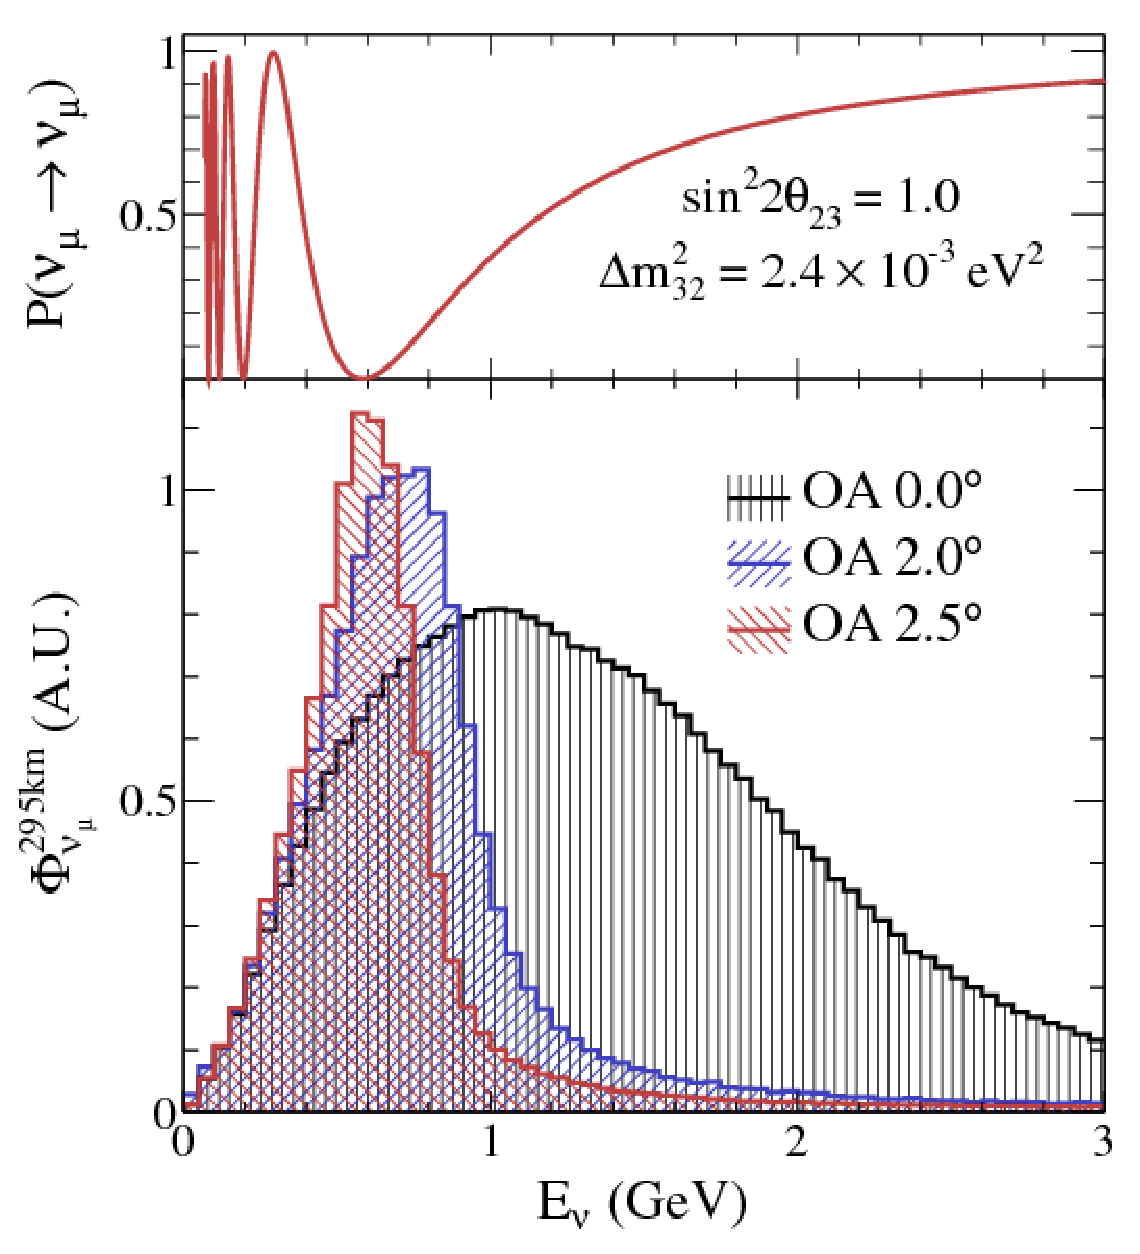
\includegraphics[width=0.8\columnwidth]{img/oaeffect_flux.eps}}
  }
  {
    % T2K detector
    \rput(0.425\slidewidth, 0.155\slideheight){\scalebox{0.75}{% T2K detector
\begin{pspicture}

  \psline[linewidth = 0.05, linecolor = pdcolor1](1.025,0)(1.025,2)
  \psline[linewidth = 0.05, linecolor = pdcolor1](2.975,0)(2.975,2)
  \psellipse[linewidth = 0.05, linecolor = pdcolor1](2,2)(1,0.2)
  \psellipse[linewidth = 0.05, linecolor = pdcolor1](2,0)(1,0.2)

  \psline[linewidth = 0.01, linecolor = pdcolor1]{|<->|}(1, -0.4)(3, -0.4)
  \rput[c](2,-0.6){\color{pdcolor1}\footnotesize $39.3$~m}
  \psline[linewidth = 0.01, linecolor = pdcolor1]{|<->|}(3.2,0)(3.2,2)
  \rput[l](3.4,1){\color{pdcolor1}\footnotesize $41.4$~m}

  \psline[linewidth = 0.03, linecolor = pdcolor4]{->}(0,1)(1.75,1)
  \rput[c](0.5,1.2){\color{pdcolor4}\footnotesize $\nu_\alpha$}

  \psline[linewidth = 0.03, linecolor = pdcolor4, linestyle = dotted]{-}(-3,1)(0,1)
  \rput[c](-1.5,1.2){\color{pdcolor4}\footnotesize 295 km}

  \psline[linewidth = 0.03, linecolor = pdcolor5]{->}(1.75,1)(2.5, 1.5)
  \rput[c]{45}(2,1.35){\color{pdcolor5}\footnotesize $\alpha$}
  \psline[linewidth = 0.03, linecolor = pdcolor3]{->}(1.75,1)(2.5, 0.75)
  \psline[linewidth = 0.03, linecolor = pdcolor3]{->}(1.75,1)(2.5, 0.5)
  \psline[linewidth = 0.03, linecolor = pdcolor3]{->}(1.75,1)(2.5, 0.25)

\end{pspicture}
}}

    \mbox{}\vspace{0.225\slideheight}  
  
    \begin{itemize}

      \item Off-axis beam
      \item Cherenkov detector (Super-Kamiokande)
      \item 50 000 tons of ultra-pure water
      \item Only charged leptons and final state charged hadrons are visible
      \item The neutrino energy is unknown
      
    \end{itemize}
  }
  
\end{wideslide}

%%%%% ENERGY RECONSTRUCTION %%%%%

\begin{slide}[toc=Energy reconstruction]{The problem with neutrino energy reconstruction}
 
  % SLIDE 1
  \onslide*{1}
  {
    \rput[c](13,3.5){% QEL vertex
\begin{pspicture}
  \rput[c](0,-1.75){Quasi-elastic scattering}
  \pscoil[coilarm = 0, linewidth = 0.025, linecolor = pdcolor1, coilwidth = 0.25, coilaspect = 0]{c-c}(-1,0)(1,0)
  \rput[c](0,-0.4){\color{pdcolor1}\small $W$}
  \psframe[linestyle = none, fillstyle = solid, fillcolor = pdcolor2](-1.1,-0.03)(-0.9,0.2)
  \psframe[linestyle = none, fillstyle = solid, fillcolor = pdcolor2](0.9,-0.03)(1.1,0.2)
  \pscircle[linestyle = none, fillstyle = solid, fillcolor = pdcolor1](-0.95,0){0.05}
  \pscircle[linestyle = none, fillstyle = solid, fillcolor = pdcolor1](0.95,0){0.05}
  \psline[linewidth = 0.025, linecolor = pdcolor1]{c-}(-0.95,0)(-2,1)
  \psline[linewidth = 0.025, linecolor = pdcolor1]{c-}(-0.95,0)(-2,-1)
  \psline[linewidth = 0.05, linecolor = pdcolor1]{c-}(0.95,0)(2,1)
  \psline[linewidth = 0.05, linecolor = pdcolor1]{c-}(0.95,0)(2,-1)
  
  \rput[l](-1.75,1){\color{pdcolor1} $l (k')$}
  \rput[l](-1.75,-1){\color{pdcolor1} $\nu (k)$}
  \rput[r](1.75,1){\color{pdcolor1} $p (p')$}
  \rput[r](1.75,-1){\color{pdcolor1} $n (p)$}

\end{pspicture}
}
    
    \mbox{} \\ \mbox{} \\
    
    In the case of neutrino scattering off \\ nucleon at rest neutrino energy can be \\ calculated from lepton kinematics:
    
    \mbox{} \\
    
    \twocolumn
    {
      \begin{eqnarray*}
	M_p^2 & = & p'^2 = (p + k - k')^2 \\ & & \\
	M_p^2 & = & m_l^2 + M_n^2 - 2M_nE_l \\
	& + & 2E_\nu(M_n - E_l + |\vec p_l|\cos\theta_l) \\ & & \\
	E_\nu & = & \frac{M_p^2 - M_n^2 - m_l^2 + 2M_nE_l}{2(M_n - E_l + |\vec p_l|\cos\theta_l)}
      \end{eqnarray*}
    }
    {
      \mbox{} \\ \mbox{} \\ \mbox{} \\
      \begin{eqnarray*}
	\hspace{20pt} k & = & (E_\nu, 0, 0, E_\nu) \\
	  k' & = & (E_l, \vec p_l) \\
	  p & = & (M_p, 0, 0, 0) \\
	  p' & = & p + q \\
	  q & = & k - k'       
      \end{eqnarray*}    
    }
  }
  % SLIDE 2-3 TOP
  \onslide*{2-3}
  {
    \rput(0.83\slidewidth, -0.075\slideheight){% nu-N scattering
\begin{pspicture}
      
  \rput[c](-1.5,0.3){\color{pdcolor4} $\nu$}
  \psline[linewidth = 0.03, linecolor = pdcolor4]{->}(-2,0)(0,0)
  
  \psline[linewidth = 0.03, linecolor = pdcolor1, linestyle = dotted](0,0)(3,0)
  \psarc[linewidth = 0.02, linecolor = pdcolor1, arrowscale = 0.75]{->}(0,0){2}{0}{18}
  \rput[l](2.2,0.35){\color{pdcolor1} $\theta_l$}

  
  \rput[c]{20}(1.7,0.85){\color{pdcolor5} $l$}
  \psline[linewidth = 0.03, linecolor = pdcolor5]{->}(0,0)(3,1)
  
  \rput[c]{-20}(1.8,-0.9){\color{pdcolor3} nucleon(s)}
  \psline[linewidth = 0.03, linecolor = pdcolor3]{->}(0,0)(3,-1)
  
  \rput[c]{-45}(0.13,-0.32){\color{pdcolor6} $\pi$}
  \psline[linewidth = 0.03, linecolor = pdcolor6]{->}(0,0)(0.5,-0.5)
  
  \rput[c](0,1.3){\color{pdcolor1} Nucleus}
  \onslide{2}{\pscircle[linewidth = 0.05, linecolor = pdcolor1, fillstyle = solid, fillcolor = pdcolor1](0,0){1}}
  \onslide{3}{\pscircle[linewidth = 0.05, linecolor = pdcolor1](0,0){1}}

\end{pspicture}
}
  
    \begin{itemize}
    
      \item Usually, the energy reconstruction procedure is based on quasi-elastic neutrino-nucleon scattering:
    
      $$E_\nu^{REC} = \frac{M_p^2 - (M_n - E_B)^2 - m_l^2 + 2(M_n - E_B)E_l}{2(M_n - E_B - E_l + |\vec p_l|\cos\theta_l)}$$

    \end{itemize}
  }
  % SLIDE 2
  \onslide*{2}
  {
    % COVER NUCLEUS
    \psframe[linewidth = 0.01, linecolor = pdcolor1](0,-2)(4,-1)
    \psframe[linewidth = 0.01, linecolor = pdcolor1](0,-3.1)(4,-2.1)
    \psframe[linewidth = 0.01, linecolor = pdcolor1](0,-3.2)(4,-4.2)
    % LABEL
    \rput[c](2,-1.5){\color{pdcolor1} Impulse Approximation}
    \rput[c](2,-2.6){\color{pdcolor1} No Fermi motion}
    \rput[c](2,-3.7){\color{pdcolor1} Binding Potential}
  }	
  
  \onslide*{3}
  {
    % LABEL
    \vspace{15pt}
    \psframe[linewidth = 0.01, linecolor = pdcolor1](-0.2,-2.8)(4.2,-1.2)
    \rput[c](2,-1.7){\color{pdcolor1} Never judge an event}
    \rput[c](2,-2.3){\color{pdcolor1} by its final state particles!}
  }
 
\end{slide}
